% vim:ft=tex:
%

\documentclass[12pt]{article}

\author{Arthur Oliveira de Rosso}
\title{GoBov - Sistema Web de Gerenciamento Bovino.}

\usepackage{times}
\usepackage[utf8]{inputenc}
\usepackage[T1]{fontenc}
\usepackage[alf]{abntex2cite}
\usepackage[brazil]{babel}
\usepackage[normalem]{ulem}
\usepackage{indentfirst}
\usepackage[top=3cm,left=3cm,bottom=2cm,right=2cm]{geometry}
\useunder{\uline}{\ul}{}
\usepackage{graphicx}
\graphicspath{{Images/}}

\newenvironment{citar}{\begin{changemargin}{4cm}{0cm}\fontsize{10pt}{12pt}\selectfont}{\end{changemargin}}

\begin{document}


{\textual}
\makeatletter
\begin{titlepage}
\begin{center}

INSTITUTO FEDERAL DE EDUCAÇÃO, CIÊNCIA E TECNOLOGIA 

DO RIO GRANDE DO SUL

CAMPUS CANOAS

CURSO TÉCNICO EM INFORMÁTICA INTEGRADO AO ENSINO MÉDIO

\vfill
\vfill

\@author

\vfill

\textbf{\@title}

\vfill

\textbf{Orientador:} Rodrigo Noll

\vfill

Canoas, \today

\end{center}
\newpage


\section{Proposta de Trabalho de Conclusão de Curso}

\subsection{Descrição do Problema}
Uma análise do processo de criação de bovinos em uma propriedade rural, demonstra que o ciclo de vida do animal necessita de um acompanhamento rigoroso e contínuo. Os registros de informações relativas aos animais adquirem profunda relevância uma vez que a falta de informações pode ocasionar um descontrole sanitário.

Segundo \citeonline{Marcelino16}, na bovinocultura brasileira, seja ela de corte ou de leite, devemos nos atentar para todos os fatores que possam prejudicar ou diminuir a produção do animal, como por exemplo, as doenças. Muitas  delas podem ser evitadas se os animais forem vacinados, por isso é importante que o produtor esteja sempre atento aos programas de vacinação adotados em cada região, levando em consideração a maneira mais adequada para tratar os animais, pois há vacinas que são aplicadas no rebanho todo, outras são aplicadas somente em certas categorias de animais, selecionando idade e até mesmo o sexo.

A problemática dos pecuaristas, que são o público alvo do presente trabalho, se dá no fato de que embora o registro individual dos animais seja fundamental por conter informações indispensáveis ao manejo do animal, não é essa uma prática habitual por se tratar de uma tarefa muitas vezes complicada, quando feita somente no papel.



\subsection{Proposta de solução}

Um sistema web de gerenciamento bovino, o qual possibilita ao usuário registrar seus animais de modo a otimizar o tempo gasto no registro do tratamento através de um controle de peso e remédios.

\subsection{Objetivos}

\subsubsection{Objetivo Geral}

Implementar um sistema web que visa gerenciar os animais de uma propriedade proporcionando um controle sanitário afim de possibilitar a identificação de possíveis focos de doenças e epidemias, bem como a aplicação de um controle de peso capaz de identificar os ganhos obtidos.

\subsubsection{Objetivos Específicos}

\begin{itemize}
	\item Escolher as tecnologias a serem utilizadas no sistema;
	\item Pesquisar as necessidades dos pecuaristas e de que maneira o sistema pode auxiliá-los;
	\item Modelar o sistema;
	\item Identificar as informações relevantes sobre o ciclo de vida do animal bovino;
	\item Realizar pesquisas de sistemas relacionados para identificar pontos onde há um nicho de mercado inexplorado;
	\item Implementar o sistema.
	\item Realizar testes do sistema.
	\item Avaliar o sistema na realidade dos pecuaristas.
\end{itemize}

\section{Trabalhos Relacionados}

% TODO: Nesse capitulo deve aparecer a analise que foi realizada em aplicativos, aplicações, sistemas, plataformas, sites, etc., que guardam semelhança com a proposta a ser desenvolvida no projeto.

Durante o levantamento de dados foram buscadas plataformas que trabalham de forma semelhante ao presente sistema, como por exemplo o BovControl, o JetBov e o A3Pecuária.

\subsection{BovControl}

O BovControl é uma ferramenta de coleta e análise de dados para melhorar a performance da produção de carne, leite ou genética \cite. Nele é possível manter

\newpage

\section{Modelo de requisitos}

\subsection{Diagrama de Casos de uso}

\begin{figure}[!h]
\begin{center}
\caption{Diagrama de Casos de Uso do sistema}
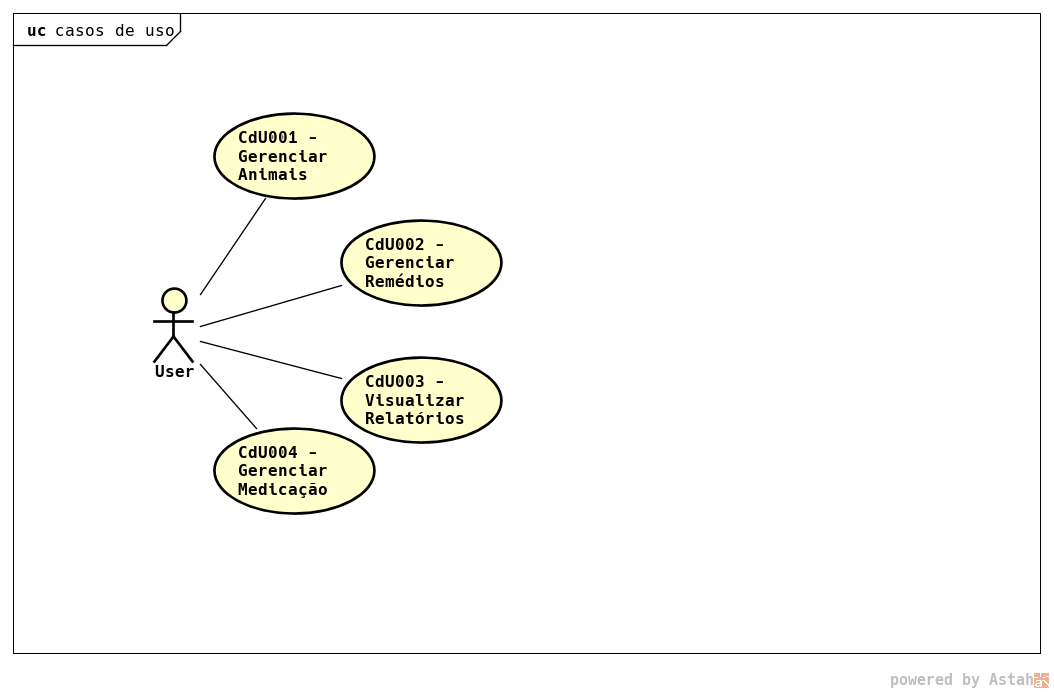
\includegraphics[width=6in]{img/casosdeuso.png}

\floatfoot{Fonte: Autoria própria.}
\end{center}
\end{figure}


\subsection{Especificação de Casos de Uso}

\begin{center}
  \begin{tabular}{ | l |  p{10cm} |}
    \hline
    Código e Nome do Caso de Uso & CdU001 - Gerenciar Animais \\ \hline
    Ator Primário: & Usuário \\ 
    Ator Secundário: & Não se aplica \\ \hline
    Fluxo Principal de Eventos & P1. O usuário solicita consultar os animais. \\
                               & P2. O sistema apresenta a tela de animais. (IV003) (A1) (A2) \\
                               & P3. O usuário solicita ver um animal em específico. \\
			       & P4. O sistema apresenta a tela de perfil do animal. (IV006) (A3) (A4)  \\
                               & P5. O caso de uso se encerra. \\ \hline
    Fluxo Alternativo:         & A1.1. Em P2 o usuário insere as informações de um animal no formulário e solicita salvá-las. \\
    A1. Adicionar animal       & A1.2. O sistema salva o animal. \\ 
			       & A1.3. Retorna ao P2. \\ \hline
    Fluxo Alternativo:         & A2.1. Em P2 o usuário tem a intenção de deletar um animal. \\
    A2. Deletar animal         & A2.2. O sistema apaga o animal selecionado. \\
			       & A2.3. Retorna ao P2. \\ \hline
    Fluxo Alternativo:         & A3.1. Em P4 o usuário decide editar animal. \\
    A3. Editar animal          & A3.2. O sistema apresenta a tela de editar animal. (IV007) \\
			       & A3.3. O usuário insere as novas informações do animal. \\
                               & A3.4. O sistema salva essas informações. \\
			       & A3.5. Retorna ao P4. \\ \hline
    Fluxo Alternativo:         & A4.1. Em P4 o decide adicionar uma nova pesagem do animal. \\
    A4. Adicionar peso         & A4.2. O sistema apresenta a tela de adicionar pesagem. (IV008) \\
			       & A4.3. O usuário insere as novas informações de peso do animal. \\
                               & A4.4. O sistema salva essas informações. \\
			       & A4.3. Retorna ao P4. \\ \hline
    Fluxo Alternativo:         & A5.1. Em P4 o usuário decide consultar detalhes do animal. \\
    A5. Consultar Detalhes     & A5.2. O sistema apresenta a tela de detalhes do animal. \\
			       & A5.3. Retorna ao P4. \\
    \hline
  \end{tabular}
\end{center}


\begin{center}
  \begin{tabular}{ | l |  p{10cm} |}
    \hline
    Código e Nome do Caso de Uso & CdU002 - Gerenciar Remédios \\ \hline
    Ator Primário: & Usuário \\ 
    Ator Secundário: & Não se aplica \\ \hline
    Fluxo Principal de Eventos & P1. O usuário solicita consultar os remédios. \\
			       & P2. O sistema apresenta a tela de remédios. (IV004) (A1) (A2) (A3) \\
                               & P3. O caso de uso se encerra. \\ \hline
    Fluxo Alternativo:         & A1.1. Em P2 o usuário insere as informações de um remédio no formulário e solicita salvá-las. \\
    A1. Adicionar remédio      & A1.2. O sistema salva o reméio. \\ 
			       & A1.3. Retorna ao P2. \\ \hline
    Fluxo Alternativo:         & A1.1. Em P2 o usuário resolve deletar um remédio. \\
    A2. Deletar remédio        & A2.2. O sistema apaga o remédio selecionado. \\
			       & A2.3. Retorna ao P2. \\ \hline
    Fluxo Alternativo:         & A3.1. Em P2 o usuário decide editar um remédio. \\
    A3. Editar remédio         & A3.2. O sistema apresenta a tela de editar remédio. \\
			       & A3.3. O usuário insere as novas informações do remédio. \\
                               & A3.4. O sistema salva essas informações. \\
			       & A2.3. Retorna ao P2. \\
    \hline
  \end{tabular}
\end{center}


\begin{center}
  \begin{tabular}{ | l |  p{10cm} |}
    \hline
    Código e Nome do Caso de Uso & CdU003 - Visualizar relatórios \\ \hline
    Ator Primário: & Usuário \\ 
    Ator Secundário: & Não se aplica \\ \hline
    Fluxo Principal de Eventos & P1. O usuário solicita consultar os relatórios. \\
			       & P2. O sistema apresenta a tela de relatórios da fazenda. \\
                               & P3. O caso de uso se encerra. \\
    \hline
  \end{tabular}
\end{center}



\begin{center}
  \begin{tabular}{ | l |  p{10cm} |}
    \hline
    Código e Nome do Caso de Uso & CdU004 - Gerenciar medicação \\ \hline
    Ator Primário: & Usuário \\ 
    Ator Secundário: & Não se aplica \\ \hline
    Fluxo Principal de Eventos & P1. O usuário solicita consultar medicação. \\
			       & P2. O sistema apresenta a tela de medicação. (IV005) (A1) (A2) (A3) \\
                               & P3. O caso de uso se encerra. \\ \hline
    Fluxo Alternativo:         & A1.1. Em P2 o usuário insere as informações de uma medicação e solicita salvá-las. \\
    A1. Adicionar medicação    & A1.2. O sistema salva a medicação. \\ 
			       & A1.3. Retorna ao P2. \\ \hline
    Fluxo Alternativo:         & A1.1. Em P2 o usuário resolve deletar uma medicação. \\
    A2. Deletar medicação      & A2.2. O sistema apaga a medicação selecionada. \\
			       & A2.3. Retorna ao P2. \\ \hline
    Fluxo Alternativo:         & A3.1. Em P2 o usuário decide editar uma medicação. \\
    A3. Editar medicação       & A3.2. O sistema apresenta a tela de editar medicação. \\
			       & A3.3. O usuário insere as novas informações da medicação. \\
                               & A3.4. O sistema salva essas informações. \\
			       & A2.3. Retorna ao P2. \\
    \hline
  \end{tabular}
\end{center}

\newpage

\subsection{Protótipos de Tela}

\subsubsection{IV001}

\begin{figure}[!h]
\begin{center}
\caption{Login no sistema}
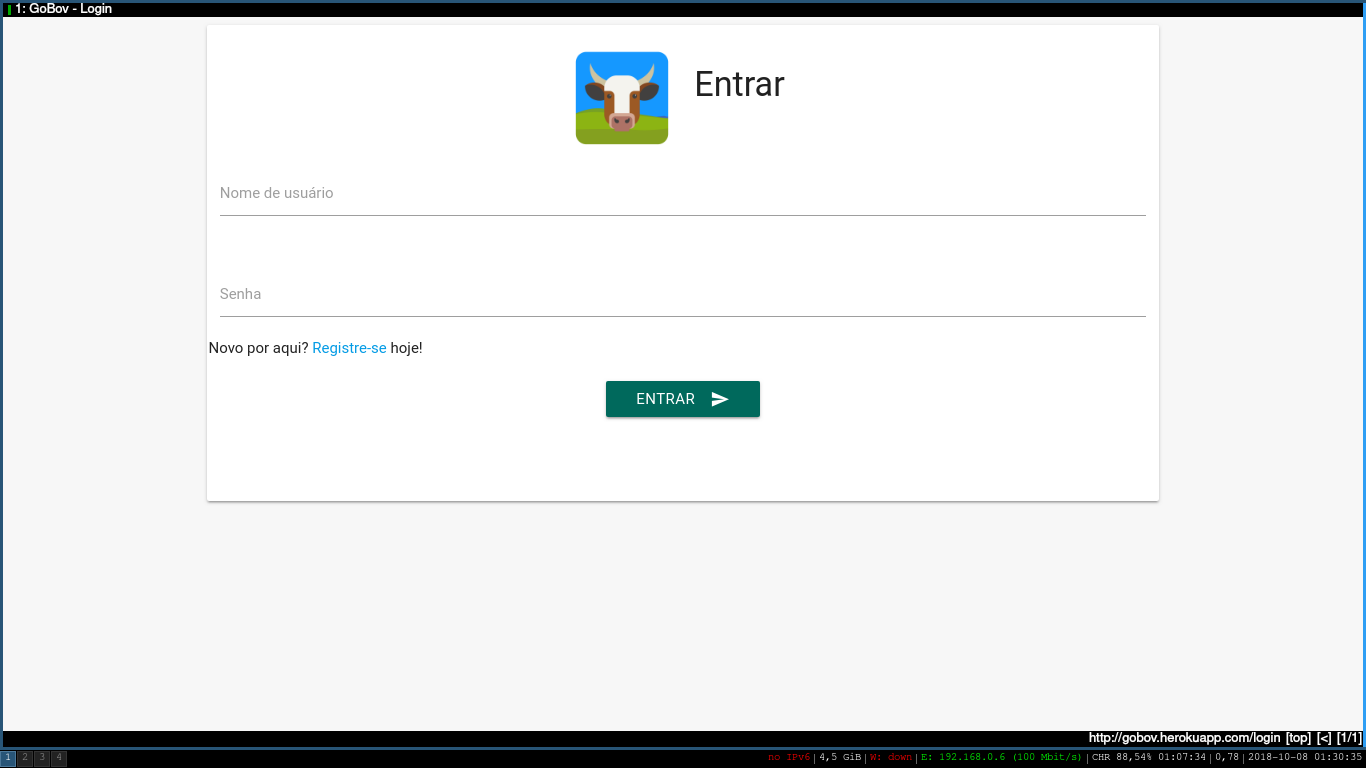
\includegraphics[width=13cm]{img/prototipos/login.png}

\floatfoot{Fonte: Autoria própria.}

\end{center}
\end{figure}


\subsubsection{IV002}

\begin{figure}[!h]
\begin{center}
\caption{Página inicial do sistema}
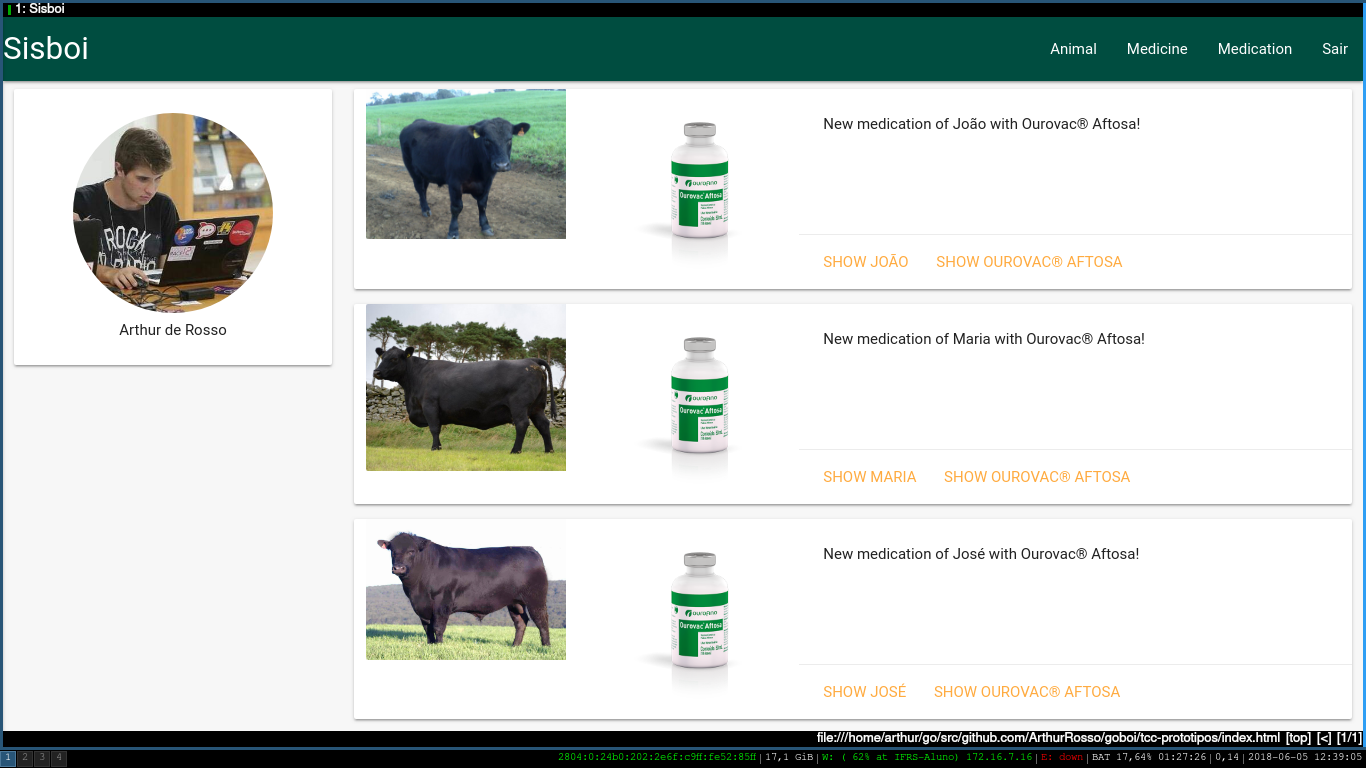
\includegraphics[width=13cm]{img/prototipos/index.png}

\floatfoot{Fonte: Autoria própria.}

\end{center}
\end{figure}

\newpage

\subsubsection{IV003}

\begin{figure}[!h]
\begin{center}
\caption{Página do animal}
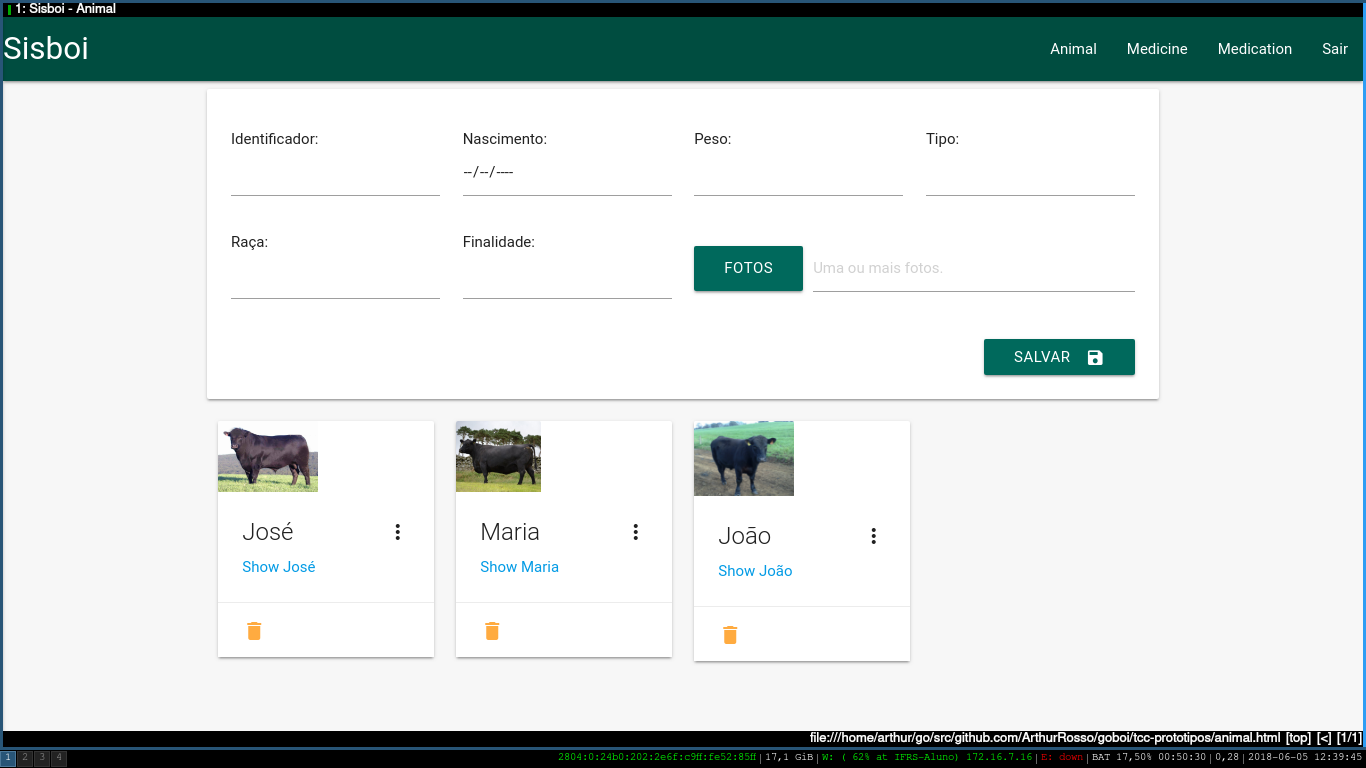
\includegraphics[width=13cm]{img/prototipos/animal.png}

\floatfoot{Fonte: Autoria própria.}

\end{center}
\end{figure}


\subsubsection{IV004}

\begin{figure}[!h]
\begin{center}
\caption{Página de remédios}
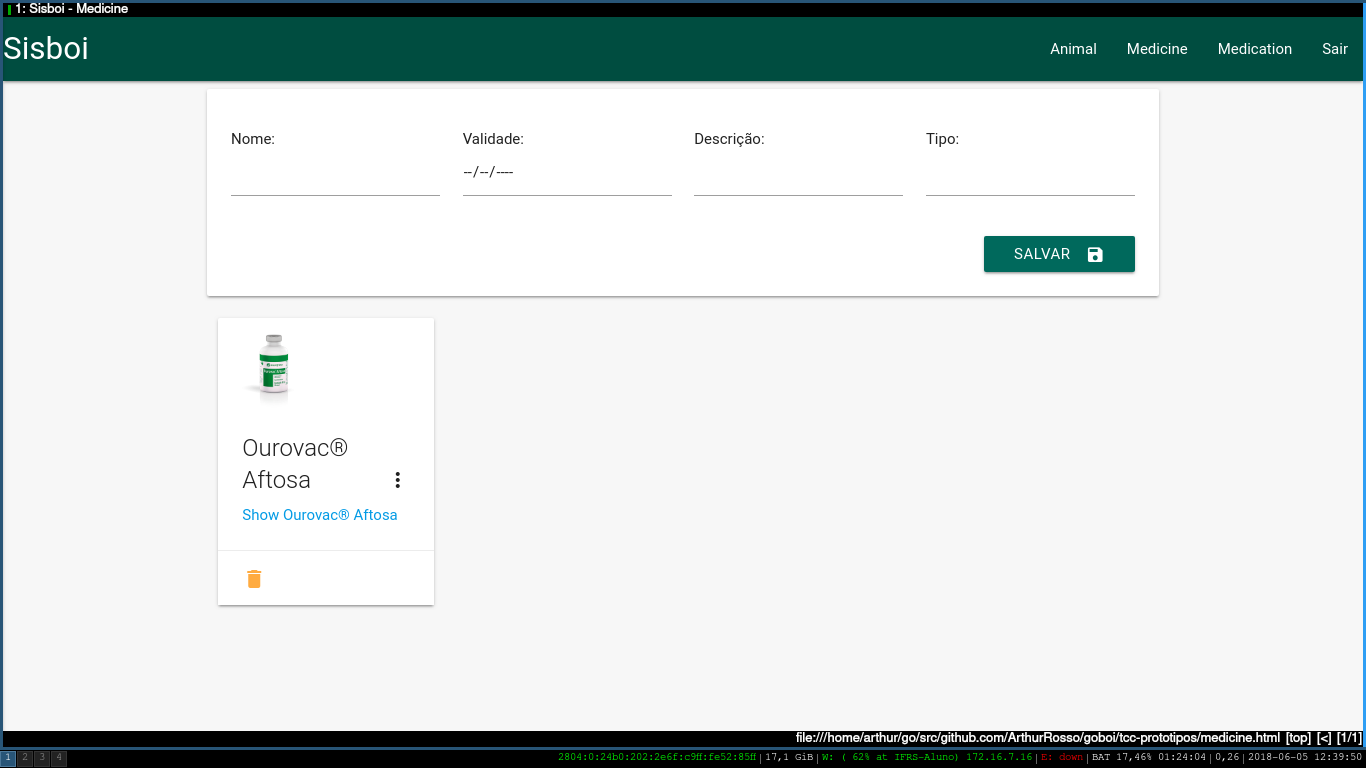
\includegraphics[width=13cm]{img/prototipos/remedio.png}

\floatfoot{Fonte: Autoria própria.}

\end{center}
\end{figure}

\newpage

\subsubsection{IV005}

\begin{figure}[!h]
\begin{center}
\caption{Página de medicação}
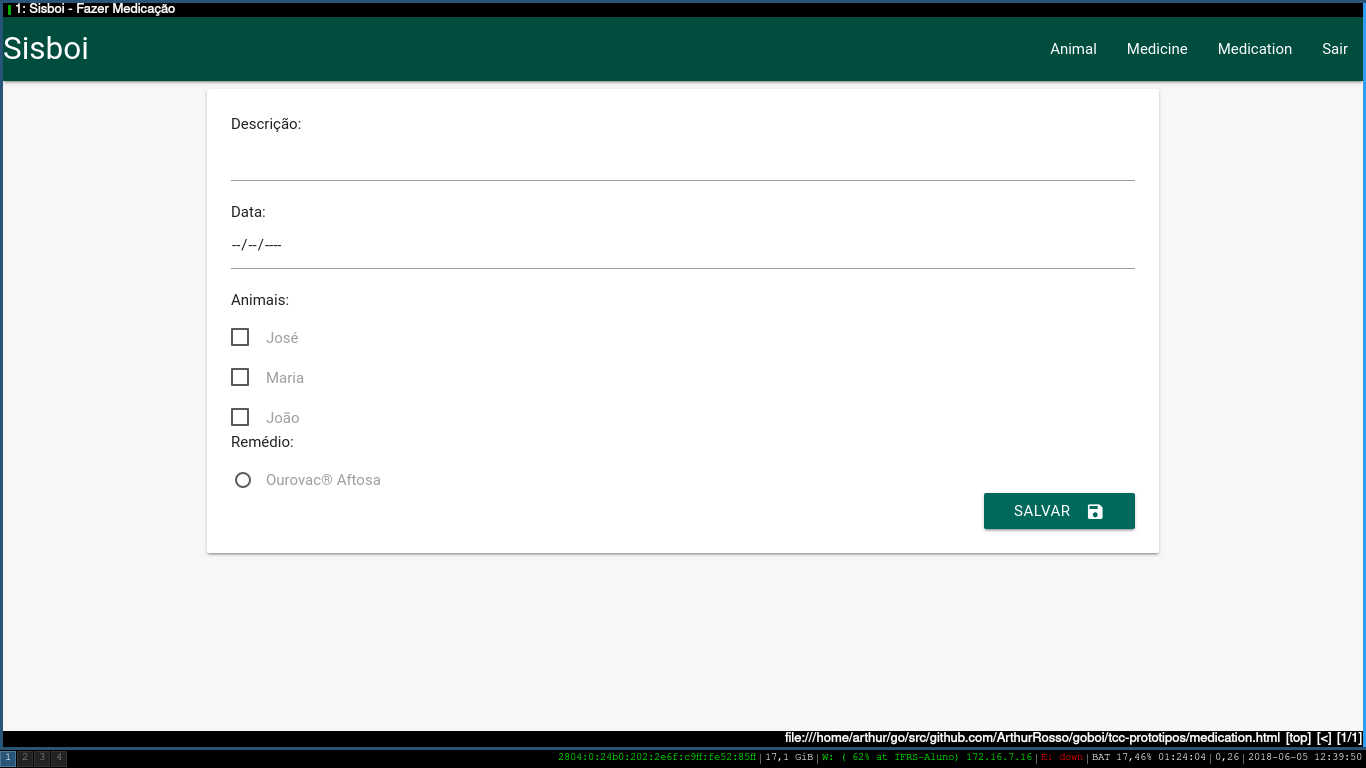
\includegraphics[width=13cm]{img/prototipos/medicacao.png}

\floatfoot{Fonte: Autoria própria.}

\end{center}
\end{figure}


\subsubsection{IV006}

\begin{figure}[!h]
\begin{center}
\caption{Página de perfil do animal}
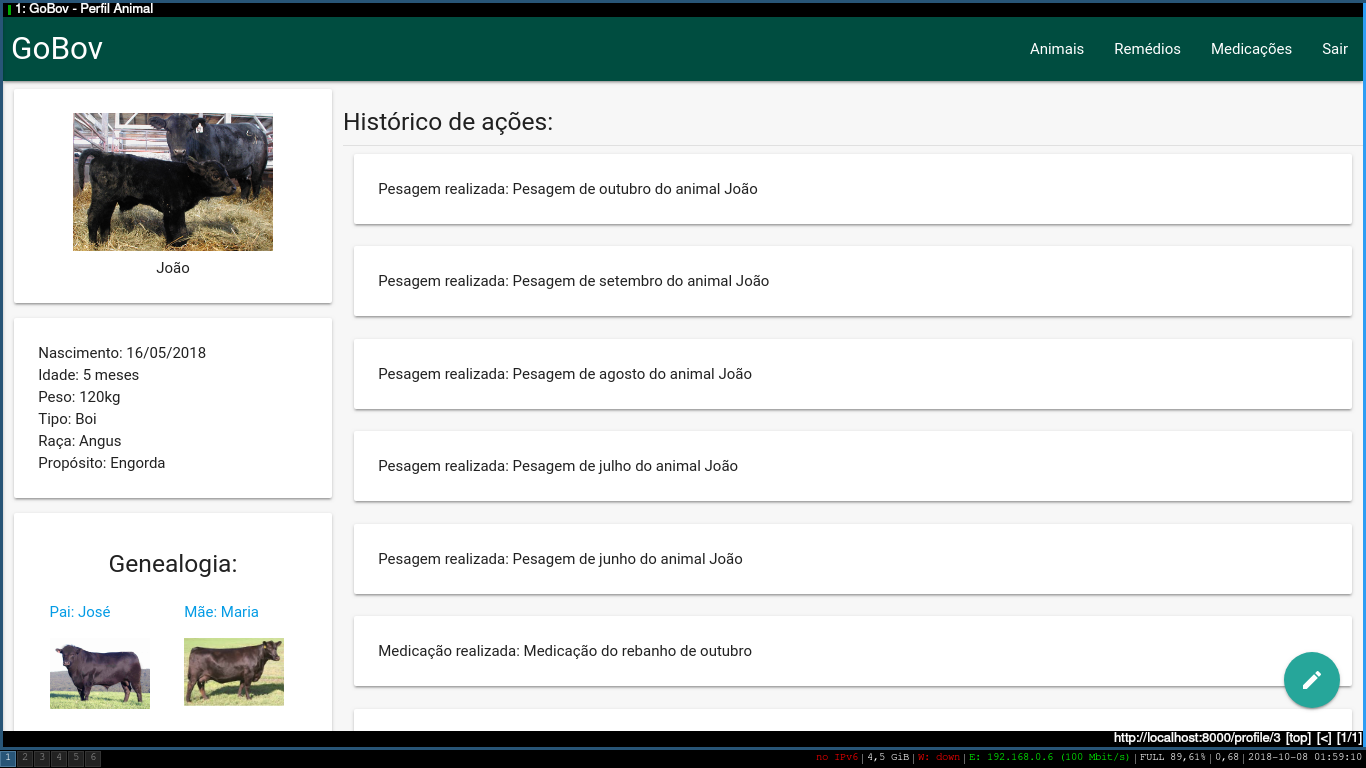
\includegraphics[width=13cm]{img/prototipos/perfil.png}

\floatfoot{Fonte: Autoria própria.}

\end{center}
\end{figure}

\newpage

\subsubsection{IV007}

\begin{figure}[!h]
\begin{center}
\caption{Página de edição do animal}
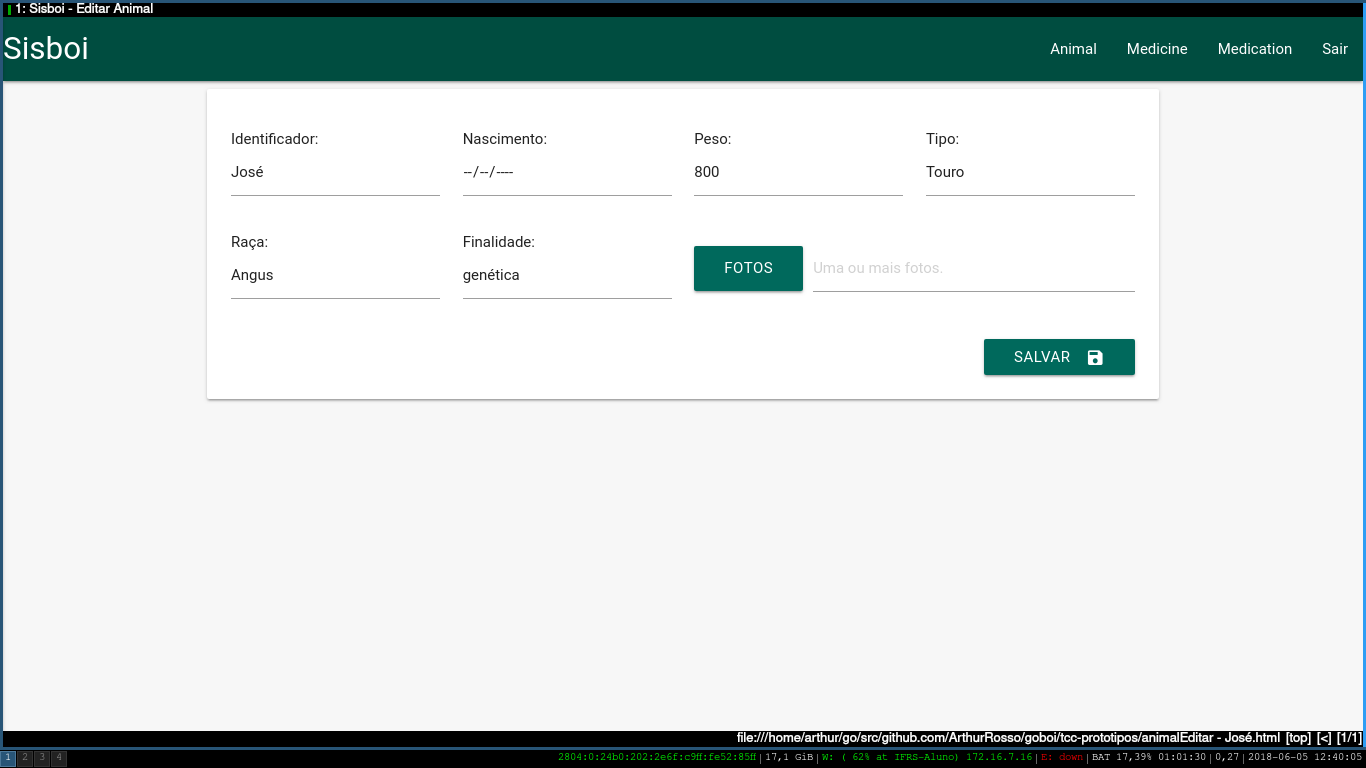
\includegraphics[width=13cm]{img/prototipos/editar.png}

\floatfoot{Fonte: Autoria própria.}

\end{center}
\end{figure}


\subsubsection{IV008}

\begin{figure}[!h]
\begin{center}
\caption{Página de pesagem do animal}
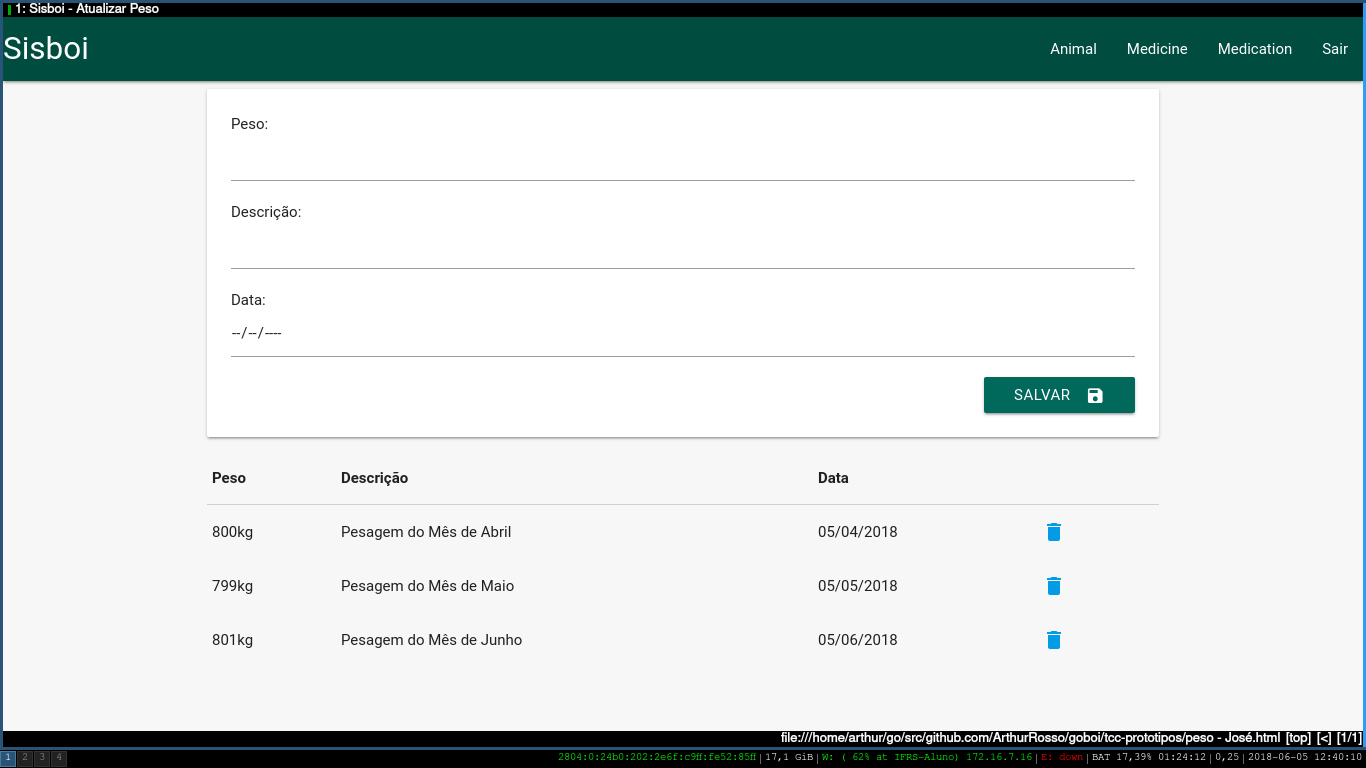
\includegraphics[width=13cm]{img/prototipos/peso.png}

\floatfoot{Fonte: Autoria própria.}

\end{center}
\end{figure}


\newpage
\section{Modelagem do Sistema}

\subsection{Diagramas de Atividade}

\begin{figure}[!h]
\begin{center}
\caption{Diagrama da Atividade de Gerenciar Animal}
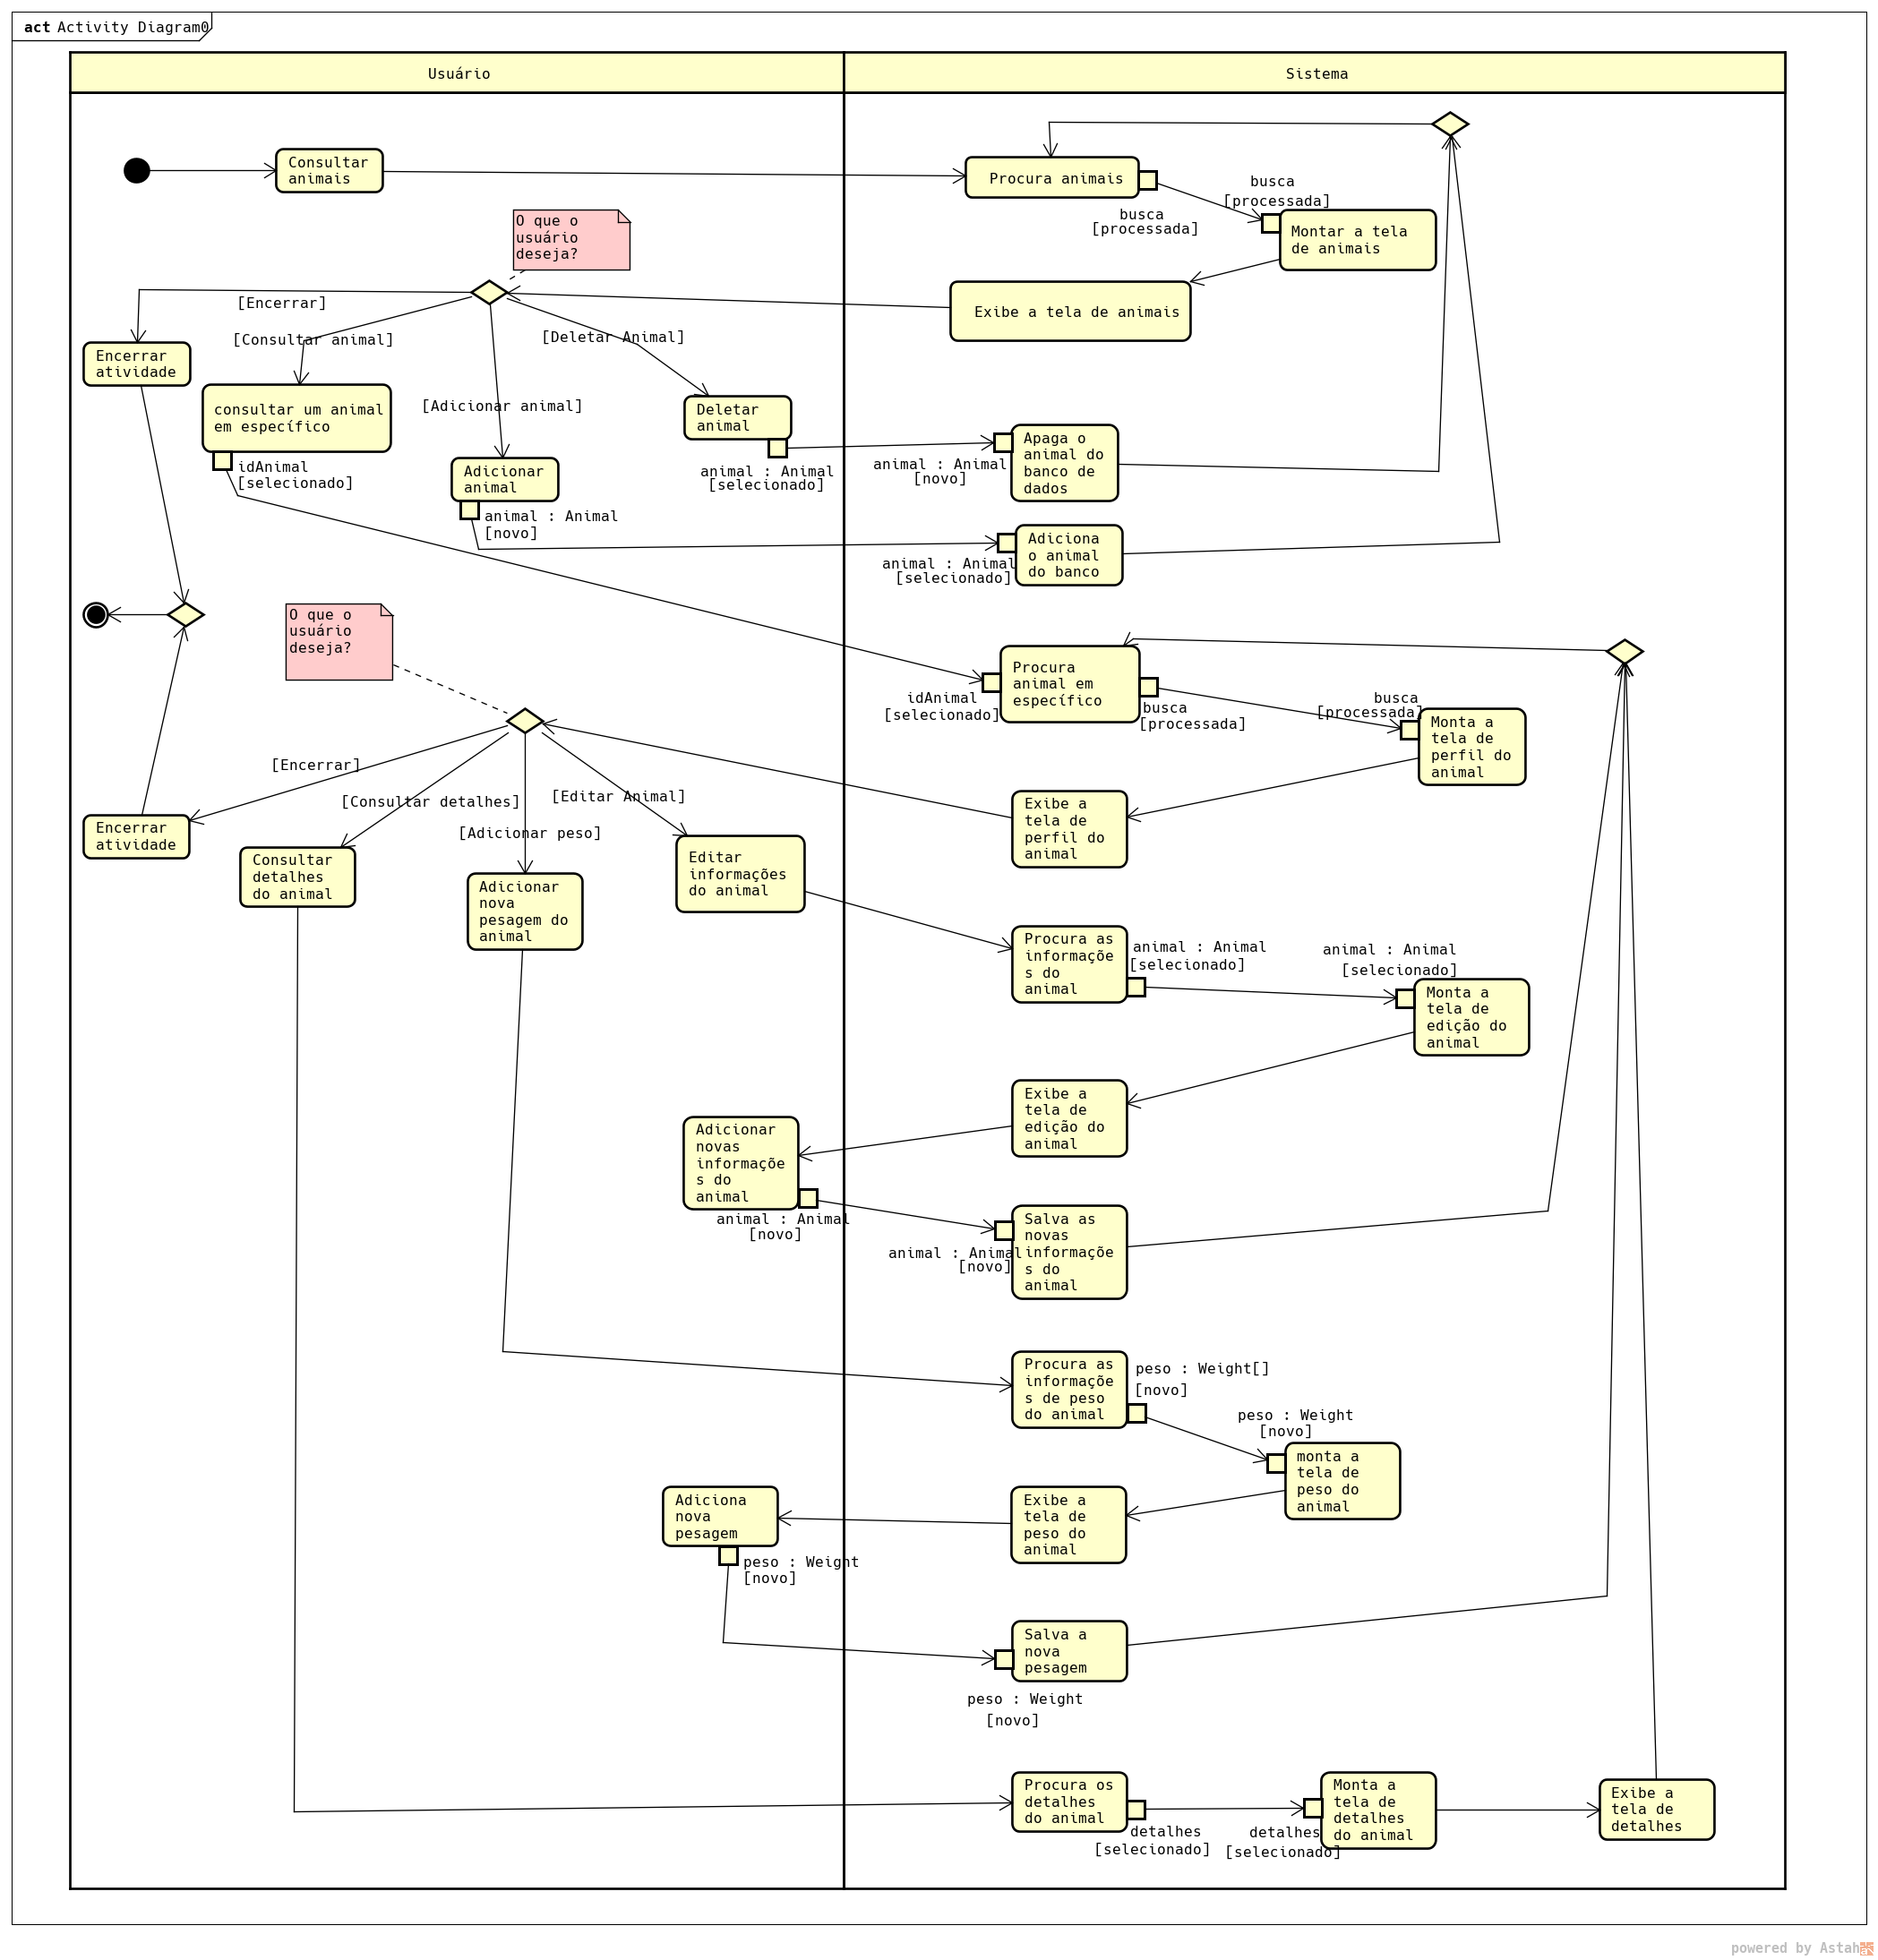
\includegraphics[width=6in]{img/atividadegerenciarboi.png}

\floatfoot{Fonte: Autoria própria.}
\end{center}
\end{figure}

\subsection{Modelagem do Banco de Dados}

\begin{figure}[!h]
\begin{center}
\caption{Modelo ER}
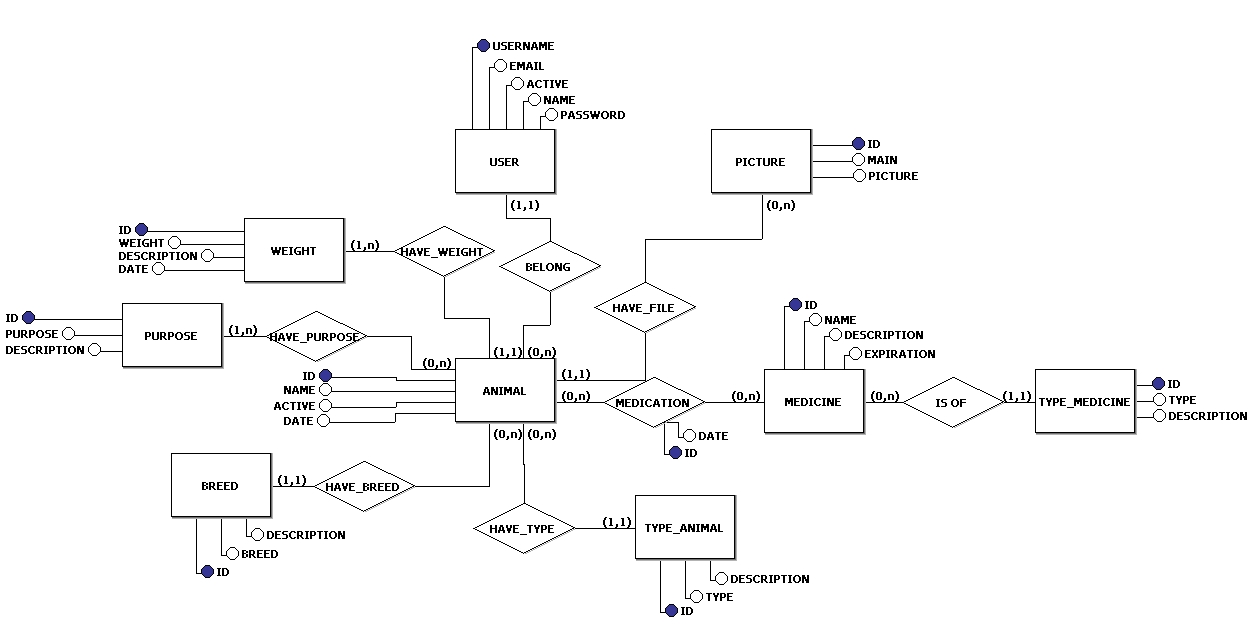
\includegraphics[width=6in]{img/erdoboi.jpeg}

\floatfoot{Fonte: Autoria própria.}

\end{center}
\end{figure}

\newpage

\section{Proposta de Solução Tecnológica Escolhida}

\subsection{Metodologia}

% TODO: Descrever se a pesquisa e exploratória, aplicada, etc, conforme visto em aula. Descrever os procedimentos para analise de requisitos que envolveu outras pessoas.

\subsection{Tecnologias Adotadas}

\begin{itemize}
	\item Golang: https://golang.org	
	\item Mysql: https://www.mysql.com
	\item HTML: https://www.w3.org/html/
	\item CSS: https://www.w3.org/Style/CSS/
	\item JavaScript: http://www.ecma-international.org/publications/standards/Stnindex.htm
	\item Materialize: https://materializecss.com/
\end{itemize}

\subsection{Ferramentas Adotadas}

\begin{itemize}
	\item Vim: https://www.vim.org
	\item phpMyAdmin: https://www.phpmyadmin.net
\end{itemize}

\newpage

\section{Cronograma}
\begin{table}[th]
\resizebox{\textwidth}{!}{%
\begin{tabular}{|c|c|c|c|c|c|c|c|c|c|c|c|c|}
\hline
\textbf{Atividade} & \textbf{Jan} & \textbf{Fev} & \textbf{Mar} & \textbf{Abr} & \textbf{Mai} & \textbf{Jun} & \textbf{Jul} & \textbf{Ago} & \textbf{Set} & \textbf{Out} & \textbf{Nov} & \textbf{Dez} \\ \hline
\begin{tabular}[c]{@{}c@{}}Escolha\\ do Orientador\end{tabular}                  & X & & & & & & & & & & & \\ \hline
\begin{tabular}[c]{@{}c@{}}Escolha\\ do Tema\end{tabular}                        & & X & & & & & & & & & & \\ \hline
\begin{tabular}[c]{@{}c@{}}Apêndice I\end{tabular}                               & & & X & & & & & & & & & \\ \hline
\begin{tabular}[c]{@{}c@{}}Apêndice II\end{tabular}                              & & & & X & X & & & & & & & \\ \hline
\begin{tabular}[c]{@{}c@{}}Apêndice III\end{tabular}                             & & & & & X & X & & & & & & \\ \hline
\begin{tabular}[c]{@{}c@{}}Elaboração do diagrama\\ de casos de uso\end{tabular} & & & & X & & & & & & & & \\ \hline
\begin{tabular}[c]{@{}c@{}}Implementação do banco de dados\end{tabular}          & & & & X & & & & & & & & \\ \hline
\begin{tabular}[c]{@{}c@{}}Implementar CRUD de animal\end{tabular}               & & & & X & X & & & & & & & \\ \hline
\begin{tabular}[c]{@{}c@{}}Implementar CRUD de remédio\end{tabular}              & & & & & X & & & & & & & \\ \hline
\begin{tabular}[c]{@{}c@{}}Implementar CRUD de medicação\end{tabular}            & & & & & & X & & & & & & \\ \hline
\begin{tabular}[c]{@{}c@{}}Implementar painel de dados\end{tabular}              & & & & & X & X & & & & & & \\ \hline
\begin{tabular}[c]{@{}c@{}}Apresentação Parcial\end{tabular}                     & & & & & & & X & & & & & \\ \hline
\begin{tabular}[c]{@{}c@{}}Testes e Validações I\end{tabular}                    & & & & & & & & X & & & & \\ \hline
\begin{tabular}[c]{@{}c@{}}Apresentação na IFCITEC\end{tabular}                  & & & & & & & & & X & & & \\ \hline
\begin{tabular}[c]{@{}c@{}}Testes e Validações II\end{tabular}                   & & & & & & & & & & X & & \\ \hline
\begin{tabular}[c]{@{}c@{}}Apresentação Final\end{tabular}                       & & & & & & & & & & & X & \\ \hline
\end{tabular}%
}
\caption{Cronograma}
\end{table}

% \section{Conclusão}

% Deste modo, surgem alguns questionamentos: Qual a efetividade do sistema apresentado e quais os benefícios e contribuições para o usuário do sistema? Quais as consequências diante da inexistência do uso de registros do ciclo de vida animal? Tais questionamentos serão respondidos através do uso do sistema e da aplicação do mesmo.

\section{Referências}

\begingroup
\renewcommand{\section}[2]{}%
\bibliography{ApendiceIII}
\endgroup

\end{document}
